\chapter{जैवसूचना-विज्ञान और अनुक्रम विश्लेषण}\label{ch:b3:bioinformatics}

गहरे समुद्र के किसी कृमि से अभी-अभी कोई जीन अनुक्रमित करने वाला कोई
जीवविज्ञानी उसके \num{300} अमीनो अम्ल किसी वेब-प्रपत्र में चिपकाता है
और तीन सेकंड बाद जान जाता है कि वह प्रोटीन किसी मानव काइनेज़ का दूर का
चचेरा भाई है, \num{280} अवशेषों पर \qty{31}{\%} समरूपता के साथ, और इस
समानता के संयोग होने की प्रायिकता $10^{-40}$ है। उन तीन सेकंडों के पीछे
1970 का कोई गतिक-क्रमादेशन अल्गोरिद्म है, यादृच्छिक \omterm{def:b3:bioinformatics:alignment}{संरेखणों} का कोई
सांख्यिकीय सिद्धांत, हज़ारों प्रोटीन कुलों से निचोड़े गए \omterm{def:b3:bioinformatics:matrices}{प्रतिस्थापन
आव्यूह}, और कोई सौ अरब अवशेषों का आँकड़ाकोश। यह अध्याय उस डिब्बे के भीतर
के तर्क के बारे में है: दो अनुक्रम इस तरह कैसे संरेखित होते हैं कि
\omterm{def:b3:bioinformatics:alignment}{संरेखण} प्रमाणतः सर्वोत्तम हो, अंक को कुछ अर्थ कैसे दिया जाता है, किसी
मेल को किसी संयोग से कैसे पहचाना जाता है, और ऐसे जीनोम में प्रतिरूप
कैसे ढूँढ़े जाते हैं जिसे पहले किसी ने देखा ही न हो। गणित प्रारंभिक है
--- कोई पुनरावृत्ति-संबंध, कोई लघुगणक, कोई पॉइसों बंटन --- और उसे जानना
सार्थक है, क्योंकि किसी अनुक्रम-तुलना से निकाला हर निष्कर्ष उसी पर टिका है।

\section{दो अनुक्रमों को संरेखित करना}

\begin{definition}[संरेखण और अंक]\label{def:b3:bioinformatics:alignment}
\index{अनुक्रम संरेखण}\index{रिक्ति-दंड}\index{वैश्विक संरेखण}\index{स्थानिक संरेखण}
दो अनुक्रमों का \emph{संरेखण} उन्हें एक के ऊपर एक लिखता है, जिसमें
\emph{रिक्तियाँ} (--) इस तरह डाली जाती हैं कि स्तंभ किसी अवशेष को किसी
अवशेष से या किसी अवशेष को किसी रिक्ति से युग्मित करें, और कोई स्तंभ दो
रिक्तियों को युग्मित न करे। उसका \emph{अंक} स्तंभों पर लिया गया वह योग
है जिसमें अवशेषों के हर युग्म के लिए कोई प्रतिस्थापन अंक $s(a,b)$ और हर
रिक्ति के लिए कोई \emph{रिक्ति-दंड} आता है: प्रति रिक्ति-स्थिति कोई
रैखिक दंड $-d$, या, अधिक यथार्थ रूप से, कोई \emph{ऐफ़ाइन} दंड
$-d - (k-1)e$, जो $k$ रिक्तियों की किसी लड़ी के लिए है और जिसमें खोलने की लागत $d$
बढ़ाने की लागत $e$ से बड़ी होती है, क्योंकि कई अवशेषों का एक ही
अंतर्वेशन एक ही विकासात्मक घटना है। कोई \emph{वैश्विक} संरेखण दोनों
अनुक्रमों को सिरे से सिरे तक ढकता है; कोई \emph{स्थानिक} संरेखण
उपअनुक्रमों का सर्वोच्च-अंक युग्म ढूँढ़ता है और शेष को अनदेखा कर देता
है, और यही चाहिए जब कोई साझा प्रांत दो अन्यथा असंबंधित प्रोटीनों में
बैठा हो।
\end{definition}

\begin{theorem}[नीडलमैन--वुंश]\label{thm:b3:bioinformatics:nw}
\index{नीडलमैन--वुंश}\index{गतिक क्रमादेशन}\index{स्मिथ--वॉटरमैन}
मान लीजिए $x = x_{1}\dots x_{m}$ और $y = y_{1}\dots y_{n}$ हैं, और
रैखिक \omterm{def:b3:bioinformatics:alignment}{रिक्ति-दंड} $d$ है। $F(i,j)$ को उपसर्गों
$x_{1}\dots x_{i}$ और $y_{1}\dots y_{j}$ के किसी \omterm{def:b3:bioinformatics:alignment}{वैश्विक संरेखण} का
सर्वोत्तम अंक मानिए। तब $F(i,0) = -id$, $F(0,j) = -jd$, और $i,j \ge 1$ के लिए
\[
F(i,j) = \max\bigl\{\,F(i-1,j-1) + s(x_{i},y_{j}),\;
F(i-1,j) - d,\; F(i,j-1) - d\,\bigr\}.
\]
$F(m,n)$ सर्वोत्तम वैश्विक अंक है, कोई सर्वोत्तम \omterm{def:b3:bioinformatics:alignment}{संरेखण}
$(m,n)$ से पीछे की ओर उन चुनावों का अनुरेखण करके पाया जाता है जिन्होंने
हर अधिकतम दिया, और पूरी गणना में $mn$ चरण लगते हैं। \omterm{def:b3:bioinformatics:alignment}{स्थानिक संरेखण} के
लिए \emph{स्मिथ--वॉटरमैन} रूपांतर अधिकतम में चौथे विकल्प के रूप में $0$
जोड़ता है, सीमाओं को $0$ रखता है, और उत्तर सारणी की सबसे बड़ी प्रविष्टि
पर पढ़ता है।
\end{theorem}
\begin{proof}
दोनों उपसर्गों के किसी भी \omterm{def:b3:bioinformatics:alignment}{संरेखण} के अंतिम स्तंभ पर विचार कीजिए। वह तीन
में से एक है: $x_{i}$ के नीचे $y_{j}$; $x_{i}$ के नीचे रिक्ति; या
रिक्ति के नीचे $y_{j}$। उसे हटाने पर क्रमशः $(x_{1}\dots x_{i-1},
y_{1}\dots y_{j-1})$ का, $(x_{1}\dots x_{i-1}, y_{1}\dots y_{j})$ का, या
$(x_{1}\dots x_{i}, y_{1}\dots y_{j-1})$ का \omterm{def:b3:bioinformatics:alignment}{संरेखण} बचता है, जिसका अंक उस
युग्म के $F$ से अधिक नहीं; और विलोमतः उन सर्वोत्तम \omterm{def:b3:bioinformatics:alignment}{संरेखणों} में से हर एक
को संगत अंतिम स्तंभ से बढ़ाया जा सकता है। इसलिए हर प्रकार के स्तंभ पर
समाप्त होने वाला सर्वोत्तम अंक छोटे युग्म का $F$ जमा उस स्तंभ का अंक
है, और सर्वोत्तम इन तीनों में सबसे बड़ा है। सीमाएँ बाध्य हैं (किसी रिक्त
उपसर्ग के सामने केवल रिक्तियाँ ही संभव हैं)।
$i + j$ पर आगमन सारणी भर देता है; कोष्ठकों की संख्या $(m+1)(n+1)$ है।
\omterm{def:b3:bioinformatics:alignment}{स्थानिक संरेखण} के लिए अतिरिक्त विकल्प $0$ का अर्थ है ``यहाँ से नया
\omterm{def:b3:bioinformatics:alignment}{संरेखण} शुरू कीजिए'', जिससे $F(i,j)$ ऐसे \omterm{def:b3:bioinformatics:alignment}{संरेखण} का सर्वोत्तम अंक बन जाता
है जो $(i,j)$ पर \emph{समाप्त} होता है, और सर्वोत्तम \omterm{def:b3:bioinformatics:alignment}{स्थानिक संरेखण} कहीं
न कहीं समाप्त होता ही है।
\end{proof}

\begin{example}[चार-गुणा-तीन की एक सारणी]\label{ex:b3:bioinformatics:nw-example}
GAT को GCAT से संरेखित कीजिए, मेल के लिए $+1$, असंगति के लिए $-1$,
$d = 1$ के साथ। सीमाएँ ऊपर की ओर $0, -1, -2, -3, -4$ और बगल में $0, -1,
-2, -3$ हैं। पंक्ति-दर-पंक्ति भरने पर: $F(\text{G},\text{G}) = 1$,
$F(\text{G},\text{C}) = 0$, $F(\text{G},\text{A}) = -1$,
$F(\text{G},\text{T}) = -2$; $F(\text{A},\text{G}) = 0$,
$F(\text{A},\text{C}) = 0$, $F(\text{A},\text{A}) = 1$,
$F(\text{A},\text{T}) = 0$; $F(\text{T},\text{G}) = -1$,
$F(\text{T},\text{C}) = -1$, $F(\text{T},\text{A}) = 0$,
$F(\text{T},\text{T}) = 2$। सर्वोत्तम $2$ है, और पीछे की ओर अनुरेखण
--- (T,T) से विकर्ण, (A,A) से विकर्ण, फिर (G,C) से बाएँ
(G,G) तक, फिर विकर्ण --- देता है
\[
\begin{array}{c}
\texttt{G-AT}\\
\texttt{GCAT}
\end{array}
\]
तीन मेल और एक रिक्ति: $3 - 1 = 2$।
\end{example}

\begin{omfigure}
\begin{tikzpicture}[every node/.style={font=\small}, >=stealth]
  \def\dx{1.0}\def\dy{0.8}
  % headers
  \foreach \j/\c in {1/G,2/C,3/A,4/T} \node[omDef, font=\small\bfseries] at (\j*\dx+0.5,0.4) {\c};
  \foreach \i/\c in {1/G,2/A,3/T} \node[omDef, font=\small\bfseries] at (-0.5,-\i*\dy-0.4) {\c};
  % grid
  \draw[gray!60] (0,0) grid[xstep=\dx, ystep=\dy] (5*\dx,-4*\dy);
  % values
  \foreach \i/\j/\v in {0/0/0,0/1/-1,0/2/-2,0/3/-3,0/4/-4,1/0/-1,2/0/-2,3/0/-3, 1/1/1,1/2/0,1/3/-1,1/4/-2, 2/1/0,2/2/0,2/3/1,2/4/0, 3/1/-1,3/2/-1,3/3/0,3/4/2}
    \node at (\j*\dx+0.5,-\i*\dy-0.4) {$\v$};
  % traceback path highlighted
  \foreach \i/\j in {0/0,1/1,1/2,2/3,3/4} \draw[omThm, very thick] (\j*\dx+0.05,-\i*\dy-0.05) rectangle (\j*\dx+\dx-0.05,-\i*\dy-\dy+0.05);
  \draw[->, omThm, very thick, shorten >=8pt, shorten <=8pt] (4.5,-2.8) -- (3.5,-2.0);
  \draw[->, omThm, very thick, shorten >=8pt, shorten <=8pt] (3.5,-2.0) -- (2.5,-1.2);
  \draw[->, omThm, very thick, shorten >=8pt, shorten <=8pt] (2.5,-1.2) -- (1.5,-1.2);
  \draw[->, omThm, very thick, shorten >=8pt, shorten <=8pt] (1.5,-1.2) -- (0.5,-0.4);
  \node[right, align=left] at (5.6,-1.6) {$F(3,4) = 2$ से प्रतिपथन:\\विकर्ण, विकर्ण,\\बाएँ (GAT में रिक्ति), विकर्ण\\[3pt] \texttt{G-AT}\\\texttt{GCAT}};
\end{tikzpicture}

{\small GAT के सामने GCAT के लिए नीडलमैन--वुंश सारणी (मेल $+1$,
असंगति $-1$, रिक्ति $-1$)। हर कोष्ठक वहाँ समाप्त होते दोनों उपसर्गों के
लिए सर्वोत्तम अंक है; कोने से पीछे अनुरेखित लाल पथ ही सर्वोत्तम \omterm{def:b3:bioinformatics:alignment}{संरेखण} है।}
\end{omfigure}

\begin{method}[दो अनुक्रमों को संरेखित करना]\label{met:b3:bioinformatics:align}
\index{प्रतिपथन}
(1) अंकन चुनिए: प्रत्याशित अपसरण के अनुकूल कोई \omterm{def:b3:bioinformatics:matrices}{प्रतिस्थापन आव्यूह}
(अज्ञात दूरी के प्रोटीनों के लिए BLOSUM62; DNA के लिए मेल/असंगति), और
ऐफ़ाइन \omterm{def:b3:bioinformatics:alignment}{रिक्ति-दंड} (BLOSUM62 के साथ प्रायः खोलना $-11$, बढ़ाना $-1$)।
(2) वैश्विक या स्थानिक तय कीजिए: ऐसे दो अनुक्रमों के लिए वैश्विक जो
अपनी पूरी लंबाई पर समजात माने जाते हों, अन्यथा स्थानिक।
(3) पुनरावृत्ति-संबंध से सारणी भरिए, और हर कोष्ठक के लिए उस चुनाव का
संकेतक रखिए जिसने उसका अधिकतम दिया। (4) $(m,n)$ से
(वैश्विक) या अधिकतम कोष्ठक से किसी शून्य तक (स्थानिक) प्रतिपथन कीजिए,
और \omterm{def:b3:bioinformatics:alignment}{संरेखण} दाएँ से बाएँ लिखिए। (5) परिणाम को उसके कच्चे अंक से नहीं,
उसकी सांख्यिकीय सार्थकता से (नीचे) परखिए, और उसे देखिए भी: लंबी
रिक्तियाँ, कम-जटिलता की लड़ियाँ और किसी पुनरावृत्ति तक सीमित \omterm{def:b3:bioinformatics:alignment}{संरेखण}
चेतावनियाँ हैं।
\end{method}

\section{अंकन: किसी मेल का मोल क्या है}

\begin{definition}[प्रतिस्थापन आव्यूह]\label{def:b3:bioinformatics:matrices}
\index{प्रतिस्थापन आव्यूह}\index{BLOSUM}\index{PAM}\index{लघुगणकीय-संभावना अंक}
कोई \emph{प्रतिस्थापन आव्यूह} अमीनो अम्लों के हर युग्म के लिए $s(a,b)$
किसी \emph{लघुगणकीय-संभावना अंक} के रूप में देता है:
\[
s(a,b) = \frac{1}{\lambda}\,\log\frac{q_{ab}}{p_{a}\,p_{b}},
\]
जहाँ $q_{ab}$ वह बारंबारता है जिससे संबंधित प्रोटीनों के विश्वसनीय
\omterm{def:b3:bioinformatics:alignment}{संरेखणों} में $a$ और $b$ संरेखित मिलते हैं, $p_{a} p_{b}$ वह बारंबारता
है जिससे वे संयोग से युग्मित होते, और $\lambda$ ऐसा मापक है जो
प्रविष्टियों को सुविधाजनक पूर्णांक बनाने के लिए चुना जाता है। कोई धनात्मक
अंक बताता है कि वह युग्म समजातों में संयोग से अधिक बार आता है; समरूपता
अंक दुर्लभ अमीनो अम्लों के लिए सबसे बड़े होते हैं (BLOSUM62 में
ट्रिप्टोफ़ैन $+11$, सिस्टीन $+9$) और सामान्य अम्लों के लिए सबसे छोटे
(ल्यूसीन $+4$, ऐलानीन $+4$), और रूढ़िवादी प्रतिस्थापन (आइसोल्यूसीन--वैलीन $+3$)
धनात्मक अंक पाते हैं जबकि उग्र प्रतिस्थापन (ट्रिप्टोफ़ैन--ग्लाइसीन $-2$)
ऋणात्मक। \emph{PAM} आव्यूह (डेहॉफ़, 1978) निकट संबंधी प्रोटीनों से
निकाले गए और आव्यूह-गुणन से अधिक दूरियों तक बढ़ाए गए;
\emph{BLOSUM} आव्यूह (हेनिकॉफ़ और हेनिकॉफ़, 1992) किसी दी हुई समरूपता पर
गुच्छित संरेखित अनुक्रमों के खंडों में सीधे गिने गए --- BLOSUM62
\qty{62}{\%} पर के खंडों से --- और वे चूक हैं क्योंकि वे उसी दूरी पर
मापे गए, बढ़ाए नहीं गए, जिस पर उनका उपयोग होता है।
\end{definition}

\begin{proposition}[लघुगणकीय-संभावना क्यों]\label{prop:b3:bioinformatics:logodds}
\index{प्रत्याशित अंक}
किसी अंकन-योजना का उपयोग \omterm{def:b3:bioinformatics:alignment}{स्थानिक संरेखण} में करने के लिए यादृच्छिक रूप
से युग्मित किसी स्तंभ का \omterm{prop:b3:bioinformatics:logodds}{प्रत्याशित अंक}, $\sum_{a,b} p_{a} p_{b}\, s(a,b)$,
ऋणात्मक होना चाहिए, और कुछ अंक धनात्मक होने चाहिए; नहीं तो
यादृच्छिक \omterm{def:b3:bioinformatics:alignment}{संरेखण} बिना किसी सीमा के बढ़ते जाते और सर्वोच्च-अंक खंड पूरा
अनुक्रम ही होता। यह मान लेने पर, ऐसी हर योजना \emph{किन्हीं} लक्ष्य
बारंबारताओं $q_{ab}$ के लिए किसी लघुगणकीय-संभावना योजना के तुल्य है ---
वह जिन \omterm{def:b3:bioinformatics:alignment}{संरेखणों} को सर्वोत्तम पाएगी वे वही हैं जिनके अवशेष-युग्म
$q_{ab}$ की तरह बँटे हैं। इसलिए आव्यूह चुनना वह अपसरण चुनना है जिसे
पकड़ने की आशा है: निकट संबंधियों के लिए कोई आव्यूह (BLOSUM80, PAM30)
तीखे धनात्मक और कठोर ऋणात्मक अंक रखता है, दूर के संबंधियों के लिए कोई
आव्यूह (BLOSUM45, PAM250) अधिक चपटा होता है।
\end{proposition}
\admitted

\begin{example}[समरूपता, सादृश्य और गोधूलि क्षेत्र]\label{ex:b3:bioinformatics:twilight}
रिक्तियों के साथ सर्वोत्तम रूप से संरेखित दो यादृच्छिक प्रोटीन अनुक्रम
संयोग से लगभग \qtyrange{15}{20}{\%} समरूपता तक पहुँच जाते हैं। सौ
अवशेषों पर \qty{35}{\%} समरूपता से ऊपर दो प्रोटीन लगभग निश्चित रूप से
समजात हैं; \qty{20}{\%} और \qty{35}{\%} के बीच \emph{गोधूलि क्षेत्र}
है, जहाँ अकेली समरूपता निर्णय नहीं कर सकती और नीचे की सांख्यिकी को करना
पड़ता है। समजात इस क्षेत्र से बहुत नीचे भी गिर सकते हैं: हीमोग्लोबिन और
मायोग्लोबिन उपइकाइयाँ \qty{25}{\%} समरूपता साझा करती हैं, लाइसोज़ाइम और
$\alpha$-लैक्टएल्ब्युमिन \qty{40}{\%}, और एक ही वलन वाले अनेक प्रोटीन
युग्म \qty{15}{\%} से भी कम, जो केवल प्रोफ़ाइलों या संरचनाओं की तुलना
से पकड़ में आते हैं।
\end{example}

\section{किसी आँकड़ाकोश में खोजना}

\begin{definition}[BLAST]\label{def:b3:bioinformatics:blast}
\index{BLAST}\index{बीज}\index{उच्च-अंक खंड युग्म}
\num{300} अवशेषों की किसी पृच्छा को $10^{11}$ के किसी आँकड़ाकोश से पूरे
\omterm{thm:b3:bioinformatics:nw}{गतिक क्रमादेशन} द्वारा संरेखित करने में प्रति खोज $3\times 10^{13}$
कोष्ठक-अद्यतन लगेंगे। \emph{BLAST} (ऑल्टशुल और सहयोगी, 1990) थोड़ी-सी
संवेदिता देकर तीन चरणों में हज़ार गुना गति खरीदता है: (1) पृच्छा के
\emph{शब्द} (प्रोटीनों के लिए तीन अवशेष, DNA के लिए ग्यारह क्षार) और
उनके उच्च-अंक पड़ोसी सूचीबद्ध कीजिए; (2) आँकड़ाकोश में ठीक-ठीक
शब्द-मेल छानिए --- यही \emph{बीज} हैं; (3) हर बीज को दोनों दिशाओं में
बिना रिक्ति तब तक बढ़ाइए जब तक अंक अपने सर्वोत्तम से एक तय मात्रा नीचे
न गिर जाए, और \emph{उच्च-अंक खंड युग्म} (HSP) रखिए, फिर पास-पास के HSP
को किसी सँकरी पट्टी में रिक्ति-सहित \omterm{thm:b3:bioinformatics:nw}{गतिक क्रमादेशन} से जोड़िए। कोई सच्चा
समजात लगभग सदा कम-से-कम एक ठीक-ठीक तीन-अवशेष शब्द साझा करता है; कोई
संयोगी समानता शायद ही करती है, और उसे कभी बढ़ाया नहीं जाता।
\end{definition}

\begin{omfigure}
\begin{tikzpicture}[every node/.style={font=\scriptsize}, >=stealth]
  % query and database sequences as bars
  \draw[very thick, omDef] (0,2.0) -- (5,2.0); \node[left] at (-0.1,2.0) {पृच्छा};
  \draw[very thick, gray] (0,0.6) -- (11,0.6); \node[left] at (-0.1,0.6) {आँकड़ाकोश};
  % seeds
  \foreach \q/\d in {1.2/3.6, 2.8/5.2, 4.1/9.3} {
    \fill[omThm] (\q-0.15,1.9) rectangle (\q+0.15,2.1);
    \fill[omThm] (\d-0.15,0.5) rectangle (\d+0.15,0.7);
    \draw[omThm, thick] (\q,1.85) -- (\d,0.75);
  }
  \node[above] at (1.2,2.15) {शब्द}; \node[above] at (2.8,2.15) {शब्द}; \node[above] at (4.1,2.15) {शब्द};
  % extension of the first two (same diagonal) -> HSP
  \draw[<->, very thick, omMeth!70!black] (2.6,0.3) -- (6.2,0.3); \node[below] at (4.4,0.25) {बिना रिक्ति बढ़ाइए: एक HSP};
  % third seed: extension fails
  \draw[omProp, thick, dashed] (8.8,0.3) -- (9.8,0.3); \node[below, omProp] at (9.3,0.25) {अंक गिरता है: छोड़ा गया};
  \node[right, align=left] at (5.5,2.0) {1. पृच्छा के शब्द\\2. आँकड़ाकोश में ठीक मेल (बीज)\\3. बढ़ाइए, उच्च-अंक युग्म रखिए};
\end{tikzpicture}

{\small \omterm{def:b3:bioinformatics:blast}{BLAST} की युक्ति। पृच्छा और आँकड़ाकोश-प्रविष्टि के साझा छोटे
ठीक-ठीक शब्द (लाल) \omterm{def:b3:bioinformatics:blast}{बीज} हैं; हर एक को उसके विकर्ण के साथ तब तक बढ़ाया
जाता है जब तक अंक चढ़ता रहे, और केवल वही विस्तार \omterm{def:b3:bioinformatics:blast}{उच्च-अंक खंड युग्म}
बनते हैं जो ऊँचे बने रहें।}
\end{omfigure}

\begin{theorem}[किसी यादृच्छिक मेल की सांख्यिकी]\label{thm:b3:bioinformatics:evalue}
\index{E-मान}\index{बिट अंक}\index{कार्लिन--ऑल्टशुल}
लंबाई $m$ की किसी पृच्छा को कुल लंबाई $n$ के किसी आँकड़ाकोश के सामने
ऋणात्मक \omterm{prop:b3:bioinformatics:logodds}{प्रत्याशित अंक} वाली किसी अंकन-योजना से खोजा जाए, तो कम-से-कम
$S$ अंक पाने वाले ऐसे बिना-रिक्ति \omterm{def:b3:bioinformatics:alignment}{स्थानिक संरेखणों} की संख्या जो संयोग से
उठते हैं, इस माध्य के साथ पॉइसों-वितरित है
\[
E = K\,m\,n\,e^{-\lambda S},
\]
जहाँ $\lambda$ और $K$ केवल अंकन-योजना और अवशेष-बारंबारताओं पर निर्भर
हैं ($\lambda$ लघुगणकीय-संभावना आव्यूह का मापक है)।
$E$ अंक $S$ का \emph{अपेक्षा-मान} है। अंक को
\emph{बिटों} में लिखने पर, $S' = (\lambda S - \ln K)/\ln 2$, सूत्र
$E = m n\, 2^{-S'}$ बन जाता है, और इसकी प्रायिकता कि कम-से-कम एक संयोगी
\omterm{def:b3:bioinformatics:alignment}{संरेखण} $S$ तक पहुँचे, $P = 1 - e^{-E}$ है, जो $E$ के छोटे होने पर $E$
के बराबर हो जाती है।
\end{theorem}
\begin{proof}[आंशिक प्रमाण]
चरघातांकी पुच्छ कार्लिन--ऑल्टशुल प्रमेय है और उसे मान लिया जाता है:
ऋणात्मक अपवाह वाले किसी यादृच्छिक चरण-पथ के अधिकतम खंड-अंक का ऐसा
बंटन होता है जिसकी पुच्छ $e^{-\lambda S}$ की तरह क्षीण होती है, जिसमें
$\lambda$ समीकरण $\sum_{a,b} p_{a} p_{b} e^{\lambda s(a,b)} = 1$ का
धनात्मक मूल है --- और यही वह समीकरण है जो लघुगणकीय-संभावना आव्यूह को
संगत बनाता है। वह पुच्छ मान लेने पर शेष केवल गिनती है। उच्च-अंक खंड
स्थितियों के $mn$ युग्मों में से किसी पर भी आरंभ हो सकते हैं, वे दुर्लभ
हैं, और वे लगभग स्वतंत्र हैं; इसलिए $S$ से आगे जाने वालों की संख्या ऐसे
माध्य के साथ पॉइसों है जो $mn$ के और पुच्छ-प्रायिकता के समानुपाती है,
$E = Kmn\,e^{-\lambda S}$। एक भी न होने की प्रायिकता $e^{-E}$ है।
बिट-अंक प्रतिस्थापन बीजगणित है: $e^{-\lambda S} K = 2^{-(\lambda S -
\ln K)/\ln 2}$। रिक्ति-सहित \omterm{def:b3:bioinformatics:alignment}{संरेखणों} के लिए वही रूप चलता है, जिसमें $\lambda$
और $K$ का आकलन अनुरूपण से होता है।
\end{proof}

\begin{example}[कोई E-मान पढ़ना]\label{ex:b3:bioinformatics:evalue}
$5\times 10^{10}$ अवशेषों के किसी आँकड़ाकोश के सामने \num{250} अवशेषों
की किसी पृच्छा का $mn = 1.25\times 10^{13} \approx 2^{43.5}$ है। जिस मेल
का \omterm{thm:b3:bioinformatics:evalue}{बिट अंक} $60$ है उसका $E = 2^{43.5 - 60} = 2^{-16.5} \approx 10^{-5}$ है:
वह मूलतः निश्चित रूप से कोई समजात है। जिस मेल का $S' = 40$ है उसका $E = 2^{3.5}
\approx 11$ है: संयोग से ऐसे ग्यारह अंक प्रत्याशित हैं, और उस मेल का
कोई अर्थ नहीं। \emph{वही} \omterm{def:b3:bioinformatics:alignment}{संरेखण}, उसी \omterm{thm:b3:bioinformatics:evalue}{बिट अंक} के साथ, दस गुना बड़े
आँकड़ाकोश में खोजा जाए तो उसका $E$ दस गुना बड़ा होता है --- सार्थकता
खोज का गुण है, उस युग्म का नहीं।
किसी विश्वसनीय समजात के लिए प्रचलित देहली $E < 10^{-3}$ है;
$E \approx 0.01$--$1$ किसी प्रोफ़ाइल-विधि से दुबारा देखने योग्य है।
\end{example}

\begin{omfigure}
\begin{tikzpicture}
\begin{axis}[
  width=0.7\linewidth, height=5.6cm,
  axis x line=bottom, axis y line=left,
  xmin=25, xmax=70, ymin=0.000000001, ymax=100000000, ymode=log,
  xlabel={बिट अंक $S'$}, ylabel={$E$},
  xlabel style={font=\small, at={(axis description cs:0.5,-0.12)}, anchor=north},
  ylabel style={font=\small},
  tick label style={font=\small}, xtick={30,40,50,60,70},
  clip=false,
]
\addplot[very thick, omDef, domain=25:70, samples=2] {2^(43.5-x)};
\addplot[very thick, omThm, domain=25:70, samples=2] {2^(46.8-x)};
\addplot[dashed, gray, domain=25:70, samples=2] {0.001};
\node[font=\scriptsize, gray, anchor=south west] at (axis cs:25.5,0.0012) {$E = 10^{-3}$};
\node[font=\scriptsize, omDef, anchor=north west] at (axis cs:26,0.00002) {$mn = 1.25\times 10^{13}$};
\node[font=\scriptsize, omThm, anchor=south west] at (axis cs:45,30) {$mn$ दस गुना बड़ा};
\end{axis}
\end{tikzpicture}

{\small $E = mn\,2^{-S'}$: हर अतिरिक्त बिट संयोगी मेलों की प्रत्याशित
संख्या आधी कर देता है, और दस गुना बड़ा आँकड़ाकोश उसी \omterm{def:b3:bioinformatics:alignment}{संरेखण} के लिए
सार्थकता के $3.3$ बिट ले लेता है।}
\end{omfigure}

\section{प्रोफ़ाइल, गुप्त अवस्थाएँ और अभिप्ररूप}

\begin{definition}[बहु-संरेखण और प्रोफ़ाइल]\label{def:b3:bioinformatics:msa}
\index{बहु-अनुक्रम संरेखण}\index{प्रोफ़ाइल}\index{प्रोफ़ाइल गुप्त मार्कोव प्रतिरूप}
कोई \emph{बहु-अनुक्रम \omterm{def:b3:bioinformatics:alignment}{संरेखण}} अनुक्रमों के किसी कुल को समजात अवशेषों के
स्तंभों में सजाता है। $k$ अनुक्रमों पर ठीक-ठीक \omterm{thm:b3:bioinformatics:nw}{गतिक क्रमादेशन} में
$n^{k}$ लागत आती है और तीन से आगे वह असंभव है; व्यावहारिक क्रमादेश
\emph{उत्तरोत्तर} संरेखित करते हैं, पहले किसी पथ-वृक्ष से निकटतम युग्म,
फिर बढ़ते \omterm{def:b3:bioinformatics:alignment}{संरेखण} में अनुक्रम और समूह, और साथ में परिष्करण की बारियाँ।
पूरा हुआ \omterm{def:b3:bioinformatics:alignment}{संरेखण} किसी \emph{प्रोफ़ाइल} के रूप में समेटा जाता है: हर
स्तंभ के लिए हर अवशेष और रिक्तियों की बारंबारता। कोई
\emph{प्रोफ़ाइल गुप्त मार्कोव प्रतिरूप} इसे मेल-अवस्थाओं की एक शृंखला
के रूप में औपचारिक बनाता है, प्रति संरक्षित स्तंभ एक, जिनमें से हर एक
अपनी ही प्रायिकताओं से अवशेष उत्सर्जित करती है, और साथ में प्रवेश तथा
विलोपन अवस्थाएँ हर स्थिति पर अतिरिक्त या अनुपस्थित अवशेषों की छूट देती
हैं; किसी कुल का प्रतिरूप (कोई Pfam प्रविष्टि) किसी नए अनुक्रम को
अवस्थाओं से होकर जाते सर्वोत्तम पथ की प्रायिकता से अंक देता है, और
युग्मवार तुलना के गोधूलि क्षेत्र से बहुत नीचे भी समजात ढूँढ़ लेता है,
क्योंकि जो स्तंभ केवल जलविरोधी अवशेष सहता है वह यह कह देता है, जबकि
कोई अकेला अनुक्रम नहीं कह सकता।
\end{definition}

\begin{omfigure}
\begin{tikzpicture}[every node/.style={font=\scriptsize}, >=stealth]
  % match states
  \foreach \i in {1,2,3,4} { \draw[thick, fill=omDef!25] (2.2*\i-0.5,0) rectangle (2.2*\i+0.5,0.7); \node at (2.2*\i,0.35) {M$_{\i}$}; }
  % insert states (diamonds) above
  \foreach \i in {1,2,3} { \draw[thick, fill=omProp!30] (2.2*\i+1.1,1.6) -- (2.2*\i+1.55,2.05) -- (2.2*\i+1.1,2.5) -- (2.2*\i+0.65,2.05) -- cycle; \node at (2.2*\i+1.1,2.05) {I$_{\i}$}; }
  % delete states (circles) below
  \foreach \i in {2,3} { \draw[thick, fill=gray!20] (2.2*\i,-1.3) circle (0.4); \node at (2.2*\i,-1.3) {D$_{\i}$}; }
  % transitions match->match
  \foreach \i in {1,2,3} \draw[->, thick] (2.2*\i+0.5,0.35) -- (2.2*\i+1.7,0.35);
  % match->insert->match
  \foreach \i in {1,2,3} { \draw[->, thick, omProp] (2.2*\i+0.3,0.7) -- (2.2*\i+0.9,1.65); \draw[->, thick, omProp] (2.2*\i+1.3,1.65) -- (2.2*\i+1.9,0.7); \draw[->, thick, omProp] (2.2*\i+1.1,2.5) arc[start angle=200, end angle=-20, radius=0.3]; }
  % match->delete->match
  \draw[->, thick, gray] (2.2+0.3,0) -- (4.4-0.3,-1.0); \draw[->, thick, gray] (4.4+0.3,-1.0) -- (6.6-0.3,0); \draw[->, thick, gray] (4.4+0.4,-1.3) -- (6.6-0.4,-1.3); \draw[->, thick, gray] (6.6+0.3,-1.0) -- (8.8-0.3,0);
  \node[below, align=center] at (2.2,-1.2) {उत्सर्जन: प्रति मेल-अवस्था\\एक अवशेष-बंटन};
  \node[right, align=left] at (9.6,1.2) {कोई अनुक्रम अपने सर्वोत्तम\\पथ से अंक पाता है: मेल,\\प्रवेश (नारंगी) और\\विलोपन (धूसर)};
\end{tikzpicture}

{\small चार स्तंभों वाले किसी कुल का \omterm{def:b3:bioinformatics:msa}{प्रोफ़ाइल गुप्त मार्कोव प्रतिरूप}।
हर मेल-अवस्था M उस स्तंभ की अपनी बारंबारताओं से कोई अवशेष उत्सर्जित
करती है; प्रवेश अवस्थाएँ I (स्व-फंदों सहित) अतिरिक्त अवशेष आने देती
हैं, विलोपन अवस्थाएँ D कोई स्तंभ छोड़ देती हैं। किसी अनुक्रम को अंक
देना उसका सर्वाधिक संभाव्य पथ ढूँढ़ना है।}
\end{omfigure}

\begin{definition}[अभिप्ररूप और सूचना-अंश]\label{def:b3:bioinformatics:motif}
\index{अभिप्ररूप}\index{स्थिति-भार आव्यूह}\index{सूचना-अंश}\index{अनुक्रम-प्रतीक}
कोई \emph{अभिप्ररूप} एक छोटा प्रतिरूप है --- कोई अनुलेखन-कारक स्थल, कोई
विच्छेदन संकेत, कोई फ़ॉस्फ़ोरिलन स्थल --- जो बारंबारताओं $f_{i}(b)$ के
किसी \emph{स्थिति-भार आव्यूह} से दर्शाया जाता है, जिसमें $b$ कोई क्षार
या अवशेष है और $i$ उसकी स्थिति। DNA के लिए स्थिति
$i$ का \emph{सूचना-अंश} $R_{i} = 2 - H_{i}$ बिट है, जहाँ $H_{i} =
-\sum_{b} f_{i}(b)\log_{2} f_{i}(b)$ उसकी एन्ट्रॉपी है: किसी अचर क्षार
के लिए $2$ बिट, और ऐसी स्थिति के लिए $0$ जहाँ चारों समान रूप से
संभाव्य हों। कुल $R = \sum_{i} R_{i}$ को किसी \emph{अनुक्रम-प्रतीक} के
रूप में खींचा जाता है, जिसमें हर स्थिति अक्षरों का ऐसा ढेर है जिसकी
कुल ऊँचाई $R_{i}$ है और जिसके अक्षरों का आकार बारंबारता से तय होता है।
\end{definition}

\begin{proposition}[किसी स्थल को कितनी सूचना चाहिए]\label{prop:b3:bioinformatics:bits}
\index{सूचना-अंश!और जीनोम आकार}
जिस स्थल को किसी जीनोम में $\gamma$ बार मिलना हो, और कहीं नहीं, और उस
जीनोम में $G$ स्थितियाँ हों, उसे लगभग $R_{\text{आवश्यक}} = \log_{2}(G/\gamma)$
बिट \omterm{def:b3:bioinformatics:motif}{सूचना-अंश} चाहिए: \omterm{def:b3:bioinformatics:motif}{अभिप्ररूप} को $G$ संभावित स्थितियों को $\gamma$
सच्ची स्थितियों तक घटाना है, और हर बिट संभावनाओं को आधा कर देता है।
भली-भाँति अध्ययन किए गए जीवाणु नियामकों के प्रेक्षित \omterm{def:b3:bioinformatics:motif}{अभिप्ररूप} इस
पूर्वानुमान से मेल खाते हैं --- \qty{4.6}{Mb} जीनोम में कुछ दर्जन जगहों
से बँधने वाले किसी दमनकारी के \emph{E.~coli} स्थल \numrange{16}{18} बिट
ढोते हैं; सुकेंद्रकी अनुलेखन-कारकों के \omterm{def:b3:bioinformatics:motif}{अभिप्ररूप}, जो $3\times 10^{9}$
जीनोम में \numrange{8}{12} बिट पर हैं, अकेले अपने लक्ष्य निर्दिष्ट नहीं
कर सकते, और इसीलिए वे संयोजनों में और
\cref{ch:b3:chromatin-epigenetics} के खुले \omterm{def:b3:chromatin-epigenetics:nucleosome}{क्रोमैटिन} में काम करते हैं।
\end{proposition}
\begin{proof}
कोई यादृच्छिक स्थिति \omterm{def:b3:bioinformatics:motif}{सूचना-अंश} $R$ वाले किसी \omterm{def:b3:bioinformatics:motif}{अभिप्ररूप} से लगभग
प्रायिकता $2^{-R}$ से मेल खाती है (विशिष्टता का हर बिट संभावना आधी कर
देता है), इसलिए $G$ स्थितियों में संयोगी मेलों की प्रत्याशित संख्या $G\,2^{-R}$ है।
सच्चे स्थलों के अलग दिखने के लिए यह $\gamma$ की कोटि का या उससे कम होना
चाहिए: $G\,2^{-R} \le \gamma$, यानी $R \ge \log_{2}(G/\gamma)$।
\end{proof}

\begin{example}[प्रत्याशित संयोगी मेल]\label{ex:b3:bioinformatics:motif-numbers}
छह नियत क्षारों वाले किसी प्रतिबंधन स्थल का $R = 12$ बिट है और वह किसी
यादृच्छिक स्थिति से प्रायिकता $4^{-6} = 2^{-12}$ से मेल खाता है: दोनों
लड़ियों पर पढ़े गए \qty{4.6}{Mb} के किसी \emph{E.~coli} जीनोम में लगभग \num{1100}
बार (स्थल तालमेलक है, इसलिए प्रति स्थिति एक बार), और मानव जीनोम में $7\times 10^{5}$
बार। जिस सुकेंद्रकी कारक के \omterm{def:b3:bioinformatics:motif}{अभिप्ररूप} में $10$ बिट हैं वह मानव जीनोम
में $3\times 10^{9}\times 2^{-10} \approx 3$ मिलियन स्थितियों से मेल
खाता है, यानी उन जीनों से कई हज़ार गुना अधिक जिनका वह नियमन करता है।
किसी बड़े जीनोम में अकेला \omterm{def:b3:bioinformatics:motif}{अभिप्ररूप} कमज़ोर पूर्वानुमानक है;
\omterm{def:b3:chromatin-epigenetics:nucleosome}{क्रोमैटिन} अवस्था, पड़ोसी \omterm{def:b3:bioinformatics:motif}{अभिप्ररूप} और जातियों के पार उस स्थल का संरक्षण
ही कोई पूर्वानुमान बनाते हैं।
\end{example}

\begin{omfigure}
\begin{tikzpicture}[every node/.style={font=\scriptsize}]
  % sequence logo: TATA box-like 8 positions, stack heights = information content (1 bit = 1 cm)
  \draw[->] (0,0) -- (0,2.2); \node[left] at (-0.05,2.0) {2}; \node[left] at (-0.05,1.0) {1}; \node[left] at (-0.05,0) {0}; \node[rotate=90, above] at (-0.55,1.1) {बिट};
  \draw (0,0) -- (8.6,0);
  \node[anchor=south, inner sep=0] at (0.5,0) {\resizebox{0.6cm}{1.9cm}{\textcolor{omThm}{\bfseries T}}};
  \node[anchor=south, inner sep=0] at (1.5,0) {\resizebox{0.6cm}{1.9cm}{\textcolor{omMeth!70!black}{\bfseries A}}};
  \node[anchor=south, inner sep=0] at (2.5,0) {\resizebox{0.6cm}{1.7cm}{\textcolor{omThm}{\bfseries T}}};
  \node[anchor=south, inner sep=0] at (3.5,0) {\resizebox{0.6cm}{1.9cm}{\textcolor{omMeth!70!black}{\bfseries A}}};
  \node[anchor=south, inner sep=0] at (4.5,0) {\resizebox{0.6cm}{1.0cm}{\textcolor{omMeth!70!black}{\bfseries A}}};
  \node[anchor=south, inner sep=0] at (4.5,1.0) {\resizebox{0.6cm}{0.4cm}{\textcolor{omThm}{\bfseries T}}};
  \node[anchor=south, inner sep=0] at (5.5,0) {\resizebox{0.6cm}{1.3cm}{\textcolor{omMeth!70!black}{\bfseries A}}};
  \node[anchor=south, inner sep=0] at (5.5,1.3) {\resizebox{0.6cm}{0.3cm}{\textcolor{omThm}{\bfseries T}}};
  \node[anchor=south, inner sep=0] at (6.5,0) {\resizebox{0.6cm}{0.5cm}{\textcolor{omProp}{\bfseries G}}};
  \node[anchor=south, inner sep=0] at (6.5,0.5) {\resizebox{0.6cm}{0.3cm}{\textcolor{omMeth!70!black}{\bfseries A}}};
  \node[anchor=south, inner sep=0] at (7.5,0) {\resizebox{0.6cm}{0.3cm}{\textcolor{omProp}{\bfseries G}}};
  \foreach \i in {1,...,8} \node[below] at (\i-0.5,-0.05) {\i};
  \node[below] at (4.3,-0.5) {स्थल में स्थिति};
\end{tikzpicture}

{\small किसी TATA-पेटी जैसे प्रवर्तक \omterm{def:b3:bioinformatics:motif}{अभिप्ररूप} का \omterm{def:b3:bioinformatics:motif}{अनुक्रम-प्रतीक}। हर
ढेर की ऊँचाई उस स्थिति का \omterm{def:b3:bioinformatics:motif}{सूचना-अंश}, $2 - H_{i}$
बिट, है; पहली चार स्थितियाँ लगभग अचर हैं और \omterm{def:b3:bioinformatics:motif}{अभिप्ररूप} के कोई $12$ बिट
में से अधिकांश ढोती हैं।}
\end{omfigure}

\section{अनुक्रम से प्रकार्य तक}

\begin{method}[किसी अज्ञात प्रोटीन पर टिप्पणी लगाना]\label{met:b3:bioinformatics:annotate}
\index{प्रांत}\index{ऑर्थोलॉगी निष्कर्षण}
कोई नया कूटलेखी अनुक्रम दिया हो तो: (1) उसे सही ढाँचे में अनूदित कीजिए
और किसी संकेत-पेप्टाइड, झिल्ली-पारी खंडों तथा कम-जटिलता क्षेत्रों की
जाँच कीजिए; (2) प्रोटीन आँकड़ाकोशों में \omterm{def:b3:bioinformatics:blast}{BLAST} से खोजिए और $E < 10^{-3}$
वाले मेल पढ़िए, यह ध्यान रखते हुए कि \omterm{def:b3:bioinformatics:alignment}{संरेखण} पूरे प्रोटीन को ढकता है
(कोई सच्चा \omterm{def:b3:genomics:comparative}{ऑर्थोलॉग}) या किसी खंड को (कोई साझा प्रांत); (3) प्रांत
आँकड़ाकोशों में \omterm{def:b3:bioinformatics:msa}{प्रोफ़ाइल} HMM से खोजिए, जो ऐसे कुल ढूँढ़ते हैं जो \omterm{def:b3:bioinformatics:blast}{BLAST}
से छूट जाते हैं और प्रोटीन को प्रांतों में बाँट देते हैं; (4) केवल
सादृश्य नहीं, ऑर्थोलॉगी निकालिए, यह जाँचकर कि दूसरे जीनोम में जो
सर्वोत्तम मेल है उसका \emph{अपना} सर्वोत्तम मेल पृच्छा है या नहीं
(पारस्परिक सर्वोत्तम मेल), या प्रोटीन को किसी जीन-वृक्ष में रखकर
(\cref{ch:b3:molecular-evolution});
(5) \omterm{def:b3:genomics:comparative}{ऑर्थोलॉगों} का प्रकार्य सावधानी से स्थानांतरित कीजिए --- कोई संरक्षित
उत्प्रेरक अवशेष संरक्षित रसायन के पक्ष में तर्क है, कोई अनुपस्थित अवशेष
विपक्ष में --- और संरचना का पूर्वानुमान कीजिए; (6) हर पूर्वानुमान को
प्रयोगशाला के लिए एक परिकल्पना मानिए।
\end{method}

\begin{proposition}[अनुक्रम से संरचना]\label{prop:b3:bioinformatics:structure}
\index{संरचना पूर्वानुमान}\index{समजातता प्रतिरूपण}\index{सहविकास}
किसी प्रोटीन का वलन उसके अनुक्रम से तय होता है
(\cref{ch:b3:structural-biology}), और अनुक्रम से उसकी गणना करना पचास
वर्षों तक इस क्षेत्र की केंद्रीय अनसुलझी समस्या रही। बारी-बारी से तीन
उपाय सफल हुए। \emph{\omterm{prop:b3:bioinformatics:structure}{समजातता प्रतिरूपण}} किसी प्रोटीन की संरचना किसी हल
हो चुके समजात की संरचना पर बनाता है, और \qty{30}{\%} समरूपता से ऊपर वह
विश्वसनीय है। \emph{सहविकास विश्लेषण} इस तथ्य का लाभ उठाता है कि वलन
में संपर्क में रहने वाले दो अवशेष किसी गहरे बहु-संरेखण के पार साथ-साथ
उत्परिवर्तित होते हैं, इसलिए सांख्यिकीय रूप से युग्मित स्तंभ-युग्म
पूर्वानुमानित संपर्क हैं, और पर्याप्त संपर्क किसी वलन को परिभाषित कर
देते हैं। लाख भर हल हो चुकी संरचनाओं और ऐसे ही \omterm{def:b3:bioinformatics:alignment}{संरेखणों} पर प्रशिक्षित
गहन-अधिगम विधियाँ अब अधिकांश गोलिकाकार प्रोटीन संरचनाओं का
पूर्वानुमान लगभग प्रायोगिक यथार्थता से कर देती हैं (2020 के CASP
आकलन), और आँकड़ाकोशों में मूलतः हर ज्ञात प्रोटीन अनुक्रम के लिए कोई
पूर्वानुमानित संरचना है। वे जो कम अच्छी तरह बताती हैं वह है जो कोई एक
संरचना पकड़ती ही नहीं: अव्यवस्थित क्षेत्र, वैकल्पिक संरूपताएँ, किसी
बिंदु उत्परिवर्तन का प्रभाव, और संकुल।
\end{proposition}

\begin{omfigure}
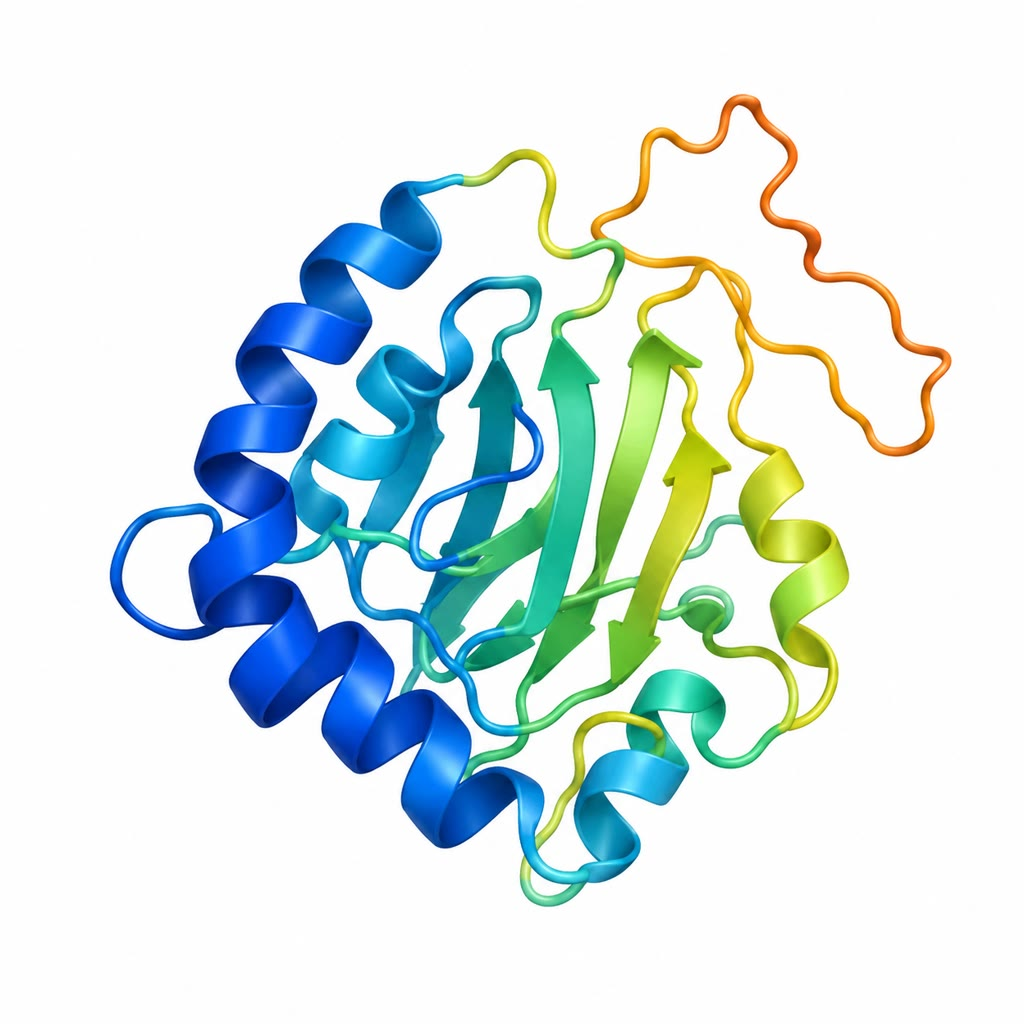
\includegraphics[width=0.36\linewidth]{images/book5/ai/b5-05-alphafold.jpg}\hspace{0.04\linewidth}
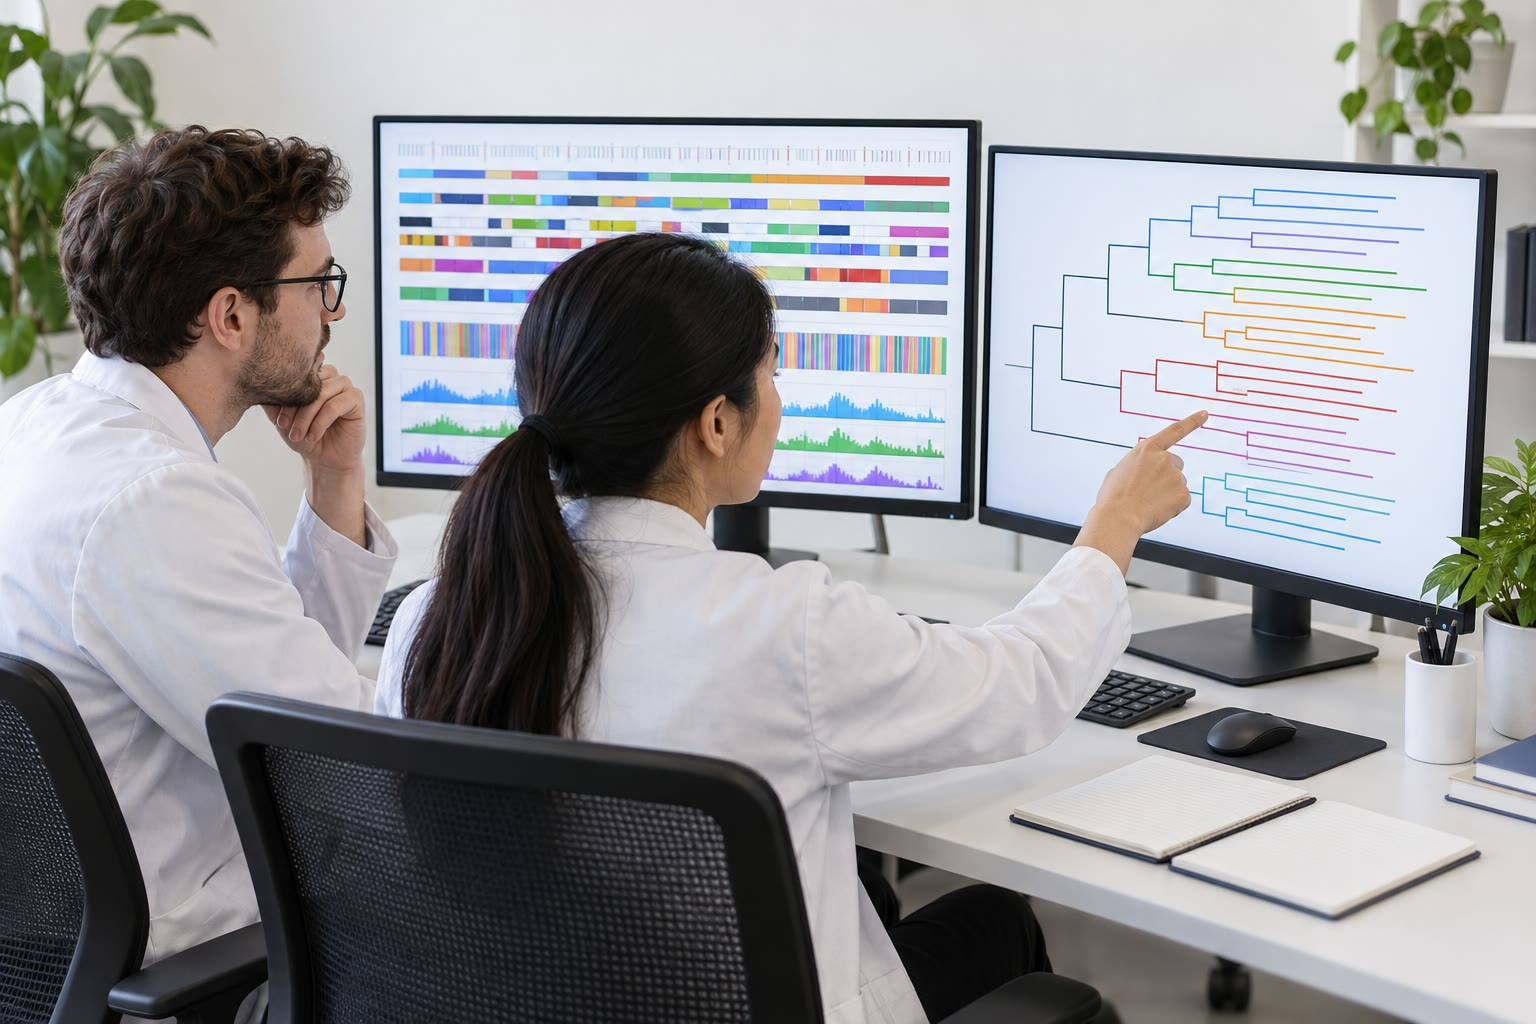
\includegraphics[width=0.54\linewidth]{images/book5/ai/b5-05-bioinformatics-lab.jpg}

{\small बाएँ: कोई पूर्वानुमानित प्रोटीन संरचना, जो प्रतिरूप के विश्वास
से रँगी है --- किसी अव्यवस्थित फंदे में ऊँचे (नीले) से नीचे (नारंगी) तक।
दाएँ: कोई जैवसूचना-विज्ञान कार्यालय --- परदों पर जीनोम-ब्राउज़र और
वृक्ष, और कोई गीली प्रयोग-मेज़ कहीं दिखती नहीं।}
\end{omfigure}

\begin{remark}[निष्कर्षण की सीमाएँ]\label{rem:b3:bioinformatics:limits}
आँकड़ाकोशों की अधिकांश प्रकार्यात्मक टिप्पणियों की कभी जाँच नहीं हुई; वे
किसी समजात से स्थानांतरित की गई थीं, और उस पर भी टिप्पणी स्थानांतरण से
ही लगी थी। त्रुटियाँ फैलती और गुणा होती हैं, और किसी भली-भाँति जुड़े
प्रोटीन पर लगी कोई गलत टिप्पणी पूरे कुल को संक्रमित कर सकती है। उपाय
वही हैं जो ऊपर दिए हैं: ऑर्थोलॉगी को समजातता से अलग कीजिए, \omterm{def:b3:bioinformatics:alignment}{संरेखण}
पढ़िए, उत्प्रेरक अवशेष ढूँढ़िए, और याद रखिए कि ``परिकल्पित प्रोटीन''
एक ईमानदार नाम है जिसके अधिकांश जीनोमों में एक-तिहाई जीन अब भी हकदार हैं।
\end{remark}

\section{अभ्यास}

\begin{exercise}[$\star$]\label{exo:b3:bioinformatics:1}
वैश्विक और \omterm{def:b3:bioinformatics:alignment}{स्थानिक संरेखण} को परिभाषित कीजिए और हर एक के लिए एक ऐसी
जैविक स्थिति दीजिए जो उसकी माँग करती हो।
\end{exercise}

\begin{exercise}[$\star$]\label{exo:b3:bioinformatics:2}
AGC के सामने AAC के लिए मेल $+1$, असंगति $-1$, रिक्ति $-1$ के साथ
नीडलमैन--वुंश सारणी भरिए, और सर्वोत्तम \omterm{def:b3:bioinformatics:alignment}{संरेखण} तथा अंक दीजिए।
\end{exercise}

\begin{exercise}[$\star$]\label{exo:b3:bioinformatics:3}
BLOSUM62 में ट्रिप्टोफ़ैन--ट्रिप्टोफ़ैन को $+11$ और ल्यूसीन--ल्यूसीन को
$+4$ अंक मिलते हैं। लघुगणकीय-संभावना सूत्र से समझाइए कि दुर्लभ अवशेष की
समरूपता का मोल अधिक क्यों है।
\end{exercise}

\begin{exercise}[$\star$]\label{exo:b3:bioinformatics:4}
E-मान क्या है? किसी खोज में $E = 3$ वाला एक मेल लौटता है। उस संख्या का
क्या अर्थ है, और क्या वह मेल कोई समजात है?
\end{exercise}

\begin{exercise}[$\star\star$]\label{exo:b3:bioinformatics:5}
\num{400} अवशेषों की किसी पृच्छा को $2\times 10^{11}$
अवशेषों के सामने खोजा जाता है। $45$, $55$ और $65$ \omterm{thm:b3:bioinformatics:evalue}{बिट अंक} वाले मेलों का
E-मान निकालिए। कौन-सा \omterm{thm:b3:bioinformatics:evalue}{बिट अंक} $E = 10^{-3}$ देता है? यदि पृच्छा
\num{40} अवशेषों की हो तो उत्तर कैसे बदलता है?
\end{exercise}

\begin{exercise}[$\star\star$]\label{exo:b3:bioinformatics:6}
ऐसे किसी \omterm{def:b3:bioinformatics:motif}{अभिप्ररूप} का \omterm{def:b3:bioinformatics:motif}{सूचना-अंश} निकालिए जिसकी चार स्थितियों पर (A, C,
G, T) की क्षार-बारंबारताएँ $(1,0,0,0)$, $(0.5,0,0.5,0)$,
$(0.25,0.25,0.25,0.25)$ और $(0.7,0.1,0.1,0.1)$ हैं। किसी \qty{4.6}{Mb}
जीनोम में उसके कितने संयोगी मेल होंगे?
\end{exercise}

\begin{exercise}[$\star\star$]\label{exo:b3:bioinformatics:7}
समझाइए कि ऐफ़ाइन \omterm{def:b3:bioinformatics:alignment}{रिक्ति-दंड} रैखिक दंडों से अधिक यथार्थ क्यों हैं, और
बहुत ऊँचा रिक्ति-खोलने का दंड तथा बहुत नीचा दंड दोनों खराब \omterm{def:b3:bioinformatics:alignment}{संरेखण}
क्यों देते हैं।
\end{exercise}

\begin{exercise}[$\star\star$]\label{exo:b3:bioinformatics:8}
किसी मानव प्रोटीन की किसी मक्खी आँकड़ाकोश के सामने की गई \omterm{def:b3:bioinformatics:blast}{BLAST} खोज
\num{600}-अवशेष पृच्छा के अवशेष 50--180 को ढकते $E = 10^{-30}$ वाला
सर्वोत्तम मेल देती है। क्या वह मक्खी प्रोटीन मानव प्रोटीन का \omterm{def:b3:genomics:comparative}{ऑर्थोलॉग}
है? आप और कौन-सी जाँच करेंगे?
\end{exercise}

\begin{exercise}[$\star\star$]\label{exo:b3:bioinformatics:9}
\omterm{def:b3:bioinformatics:msa}{प्रोफ़ाइल} विधियाँ ऐसे समजात क्यों पकड़ लेती हैं जो युग्मवार \omterm{def:b3:bioinformatics:alignment}{संरेखण} से
छूट जाते हैं? किसी ऐसे स्तंभ-प्रतिरूप का उदाहरण दीजिए जिसे कोई
\omterm{def:b3:bioinformatics:msa}{प्रोफ़ाइल} पकड़ती है और कोई अकेला अनुक्रम नहीं।
\end{exercise}

\begin{exercise}[$\star\star\star$]\label{exo:b3:bioinformatics:10}
दिखाइए कि धनात्मक \omterm{prop:b3:bioinformatics:logodds}{प्रत्याशित अंक} वाली किसी अंकन-योजना के अंतर्गत दो
लंबे यादृच्छिक अनुक्रमों के स्मिथ--वॉटरमैन \omterm{def:b3:bioinformatics:alignment}{स्थानिक संरेखण} का अंक उनकी
लंबाई के साथ रैखिक रूप से बढ़ता है, और समझाइए कि इससे E-मान सिद्धांत
क्यों विफल हो जाता है। \qty{60}{\%} GC अंश पर मेल $+1$ और असंगति $-1$
के साथ DNA संरेखित करने के लिए इसका क्या अर्थ है?
\end{exercise}

\begin{exercise}[$\star\star\star$]\label{exo:b3:bioinformatics:11}
नीडलमैन--वुंश सारणी को $mn$ स्मृति-कोष्ठक चाहिए; दो
\qty{100}{Mb} गुणसूत्रों के लिए वह $10^{16}$ है। उन दो विचारों का वर्णन
कीजिए जिनसे जीनोम-संरेखक इससे बचते हैं (\omterm{def:b3:bioinformatics:blast}{बीज} और शृंखलन; पट्टीकरण), और हर
एक क्या छोड़ देता है।
\end{exercise}

\begin{exercise}[$\star\star\star$]\label{exo:b3:bioinformatics:12}
जीवाणुओं के लिए किसी जीन-खोजी HMM में तीनों कूटक-स्थितियों और अकूटलेखी
DNA के लिए अवस्थाएँ हैं। समझाइए कि यह प्रतिरूप बिना किसी विराम-कूटक
सूचना के भी कूटलेखी और अकूटलेखी अनुक्रम में भेद कैसे कर सकता है
(कूटक-उपयोग पर विचार कीजिए), और वही उपाय मानव जीनोम में कहीं कठिन क्यों है।
\end{exercise}

\section{समस्या: गहरे समुद्र से आया एक अनुक्रम}

\begin{problem}[{सप्तांत समस्या --- कोई अज्ञात प्रोटीन हाथ से संरेखित,
आँकड़ाकोशों में खोजा गया और उसकी सार्थकता की गणना, उसके नियामक
अभिप्ररूप का बिटों में तौल, और उसके जीन की यादृच्छिक खुले वाचन-ढाँचों
की सांख्यिकी से जाँच, जिसका अंत सर्वोत्तम मेल के E-मान, किसी स्थल को
चाहिए बिटों और किसी वाचन-ढाँचे की उस लंबाई पर होता है जिस पर उस पर
विश्वास किया जा सके}]
\label{pb:b3:bioinformatics:1}
आँकड़े: गहरे समुद्र के किसी वलयकृमि का \num{300}-अवशेष प्रोटीन। प्रोटीन
आँकड़ाकोश: $1.2\times 10^{11}$ अवशेष। कृमि का जीनोम:
\qty{1.6}{Gb}, \qty{38}{\%} GC। हाथ के \omterm{def:b3:bioinformatics:alignment}{संरेखणों} के लिए अंकन: मेल $+1$,
असंगति $-1$, रिक्ति $-1$। सर्वोत्तम \omterm{def:b3:bioinformatics:blast}{BLAST} मेल का \omterm{thm:b3:bioinformatics:evalue}{बिट अंक}: $92$; दसवें
मेल का: $38$।

\medskip
\noindent\textbf{भाग I --- हाथ से।}
\begin{enumerate}
  \item KQT और KAQT पेप्टाइडों को नीडलमैन--वुंश
        पुनरावृत्ति-संबंध से संरेखित कीजिए: सारणी लिखिए और सर्वोत्तम
        \omterm{def:b3:bioinformatics:alignment}{संरेखण} तथा अंक दीजिए।
  \item ACAT के सामने GATCAT के लिए स्मिथ--वॉटरमैन (स्थानिक) से
        दोहराइए: सर्वोत्तम \omterm{def:b3:bioinformatics:alignment}{स्थानिक संरेखण} और उसका अंक ढूँढ़िए।
  \item \num{300}-अवशेष प्रोटीन का किसी \num{450}-अवशेष प्रोटीन के
        सामने \omterm{def:b3:bioinformatics:alignment}{वैश्विक संरेखण} कितने कोष्ठक-अद्यतन लेता है? पूरे
        आँकड़ाकोश के सामने?
  \item यदि कोई कंप्यूटर प्रति सेकंड $10^{9}$ अद्यतन करे, तो प्रश्न 3
        का पूरा आँकड़ाकोश-संरेखण कितना समय लेगा? इसके बजाय \omterm{def:b3:bioinformatics:blast}{BLAST} क्यों
        काम में लिया जाता है?
  \item BLOSUM62 समरूपता अंक ऐलानीन के लिए $+4$ ($p_{A} =
        0.074$) और ट्रिप्टोफ़ैन के लिए $+11$ ($p_{W} = 0.013$) है।
        $\lambda = 0.347$ (अर्ध-बिट मात्रक) के साथ लक्ष्य बारंबारता
        $q_{AA}$ और $q_{WW}$, और हर एक के लिए अनुपात $q/p^{2}$
        निकालिए। व्याख्या कीजिए।
  \item दो प्रोटीन $250$ अवशेषों पर \qty{24}{\%} समरूपता साझा करते हैं।
        बताइए कि यहाँ अकेली समरूपता समजातता का निपटारा क्यों नहीं कर
        सकती और कौन-सी बात कर सकती है।
\end{enumerate}

\medskip
\noindent\textbf{भाग II --- खोज।}
\begin{enumerate}[resume]
  \item आँकड़ाकोश के सामने पृच्छा के लिए $mn$ और
        $\log_{2}(mn)$ निकालिए।
  \item सर्वोत्तम मेल ($S' = 92$) और दसवें मेल ($S' = 38$) का
        E-मान निकालिए।
  \item इस खोज के लिए कौन-सा \omterm{thm:b3:bioinformatics:evalue}{बिट अंक} $E = 10^{-3}$ के तुल्य है?
        $E = 1$ के?
  \item आँकड़ाकोश के बढ़कर $1.2\times 10^{12}$ अवशेषों का हो जाने पर
        वही सर्वोत्तम मेल मिलता है। उसका E-मान?
  \item दसवाँ मेल पृच्छा के अवशेष 200--260 को $60$ अवशेषों पर
        \qty{40}{\%} समरूपता के साथ संरेखित करता है। E-मान का उपयोग
        करते हुए बताइए कि वह समजातता का प्रमाण है या नहीं, और कोई
        प्रोफ़ाइल-खोज क्या जोड़ सकती है।
  \item सर्वोत्तम मेल कोई मानव काइनेज़ है, जो अवशेष 10--290 पर संरेखित
        है। कृमि के प्रोटीनांश में उसका सर्वोत्तम मेल यही पृच्छा है।
        यह पारस्परिक परीक्षण क्या स्थापित करता है, और क्या नहीं?
\end{enumerate}

\medskip
\noindent\textbf{भाग III --- एक \omterm{def:b3:bioinformatics:motif}{अभिप्ररूप}।}
\begin{enumerate}[resume]
  \item जीन के ऊपर की ओर आठ स्थितियों का कोई संभावित अनुलेखन-कारक
        स्थल है, जिसके \omterm{def:b3:bioinformatics:motif}{सूचना-अंश}
        $2, 2, 1.6, 2, 0.8, 1.2, 0.4, 0.3$ बिट हैं। कुल $R$?
  \item \qty{1.6}{Gb} जीनोम में (दोनों लड़ियाँ, $3.2\times 10^{9}$
        स्थितियाँ) \omterm{def:b3:bioinformatics:motif}{अभिप्ररूप} के कितने संयोगी मेल होंगे?
  \item कारक लगभग $200$ जीनों का नियमन करता है। इस जीनोम में अकेले
        $200$ स्थल निर्दिष्ट करने के लिए किसी \omterm{def:b3:bioinformatics:motif}{अभिप्ररूप} को कितने बिट
        चाहिए होंगे?
  \item यदि दोनों को किसी नियत अंतराल के भीतर साथ आना पड़े, तो $8$ बिट
        का कोई दूसरा, सटा हुआ \omterm{def:b3:bioinformatics:motif}{अभिप्ररूप} इस कमी का कितना भाग पूरा कर
        सकता है?
  \item (A, C, G, T) के लिए बारंबारताएँ $(0.5, 0.5, 0, 0)$ रखने वाली
        कोई स्थिति: उसकी एन्ट्रॉपी और \omterm{def:b3:bioinformatics:motif}{सूचना-अंश} निकालिए।
  \item सूचना के तर्क से समझाइए कि जीवाणु अनुलेखन-कारकों के स्थल
        सुकेंद्रकी कारकों के स्थलों से प्रायः लंबे और अधिक संरक्षित
        क्यों होते हैं।
\end{enumerate}

\medskip
\noindent\textbf{भाग IV --- स्वयं जीन।}
\begin{enumerate}[resume]
  \item एकसमान क्षार-संघटन वाले यादृच्छिक DNA में इसकी प्रायिकता क्या
        है कि कोई कूटक विराम-कूटक हो? किसी विराम-कूटक के आने से पहले
        कूटकों की प्रत्याशित संख्या क्या है (कोई ज्यामितीय बंटन)?
  \item कृमि का जीनोम \qty{38}{\%} GC है। वास्तविक क्षार-बारंबारताओं
        के साथ इसकी प्रायिकता फिर से निकालिए कि कोई यादृच्छिक कूटक
        विराम-कूटक (TAA, TAG, TGA) हो, और वाचन-ढाँचे की प्रत्याशित
        लंबाई भी। कम GC अंश जीन-खोज को किस ओर धकेलता है?
  \item इसकी प्रायिकता क्या है कि कोई यादृच्छिक खुला वाचन-ढाँचा
        कम-से-कम $100$ कूटक लंबा हो? कम-से-कम $300$?
  \item \qty{1.6}{Gb} जीनोम में दो लड़ियों पर छह ढाँचे लगभग
        $3.2\times 10^{9}$ कूटक-आरंभ देते हैं। कम-से-कम $100$ कूटकों
        के कितने यादृच्छिक खुले वाचन-ढाँचे प्रत्याशित हैं? कम-से-कम
        $300$ के?
  \item समझाइए कि ``$100$ कूटकों से लंबा खुला वाचन-ढाँचा'' किसी जीवाणु
        में तो काम का जीन-खोजी है पर इस जीनोम में नहीं, और कोई
        सुकेंद्रकी जीन-खोजी इसके बजाय किसका उपयोग करता है।
  \item कृमि के जीन में छह बहिर्वेशन हैं, जो औसतन \qty{150}{bp} के
        हैं। समझाइए कि RNA अनुक्रमण के \omterm{def:b3:genomics:ngs}{वाचन} उस बहिर्वेशन-संरचना को
        कैसे सुलझा देते हैं जिसे अकेला जीनोमी अनुक्रम अस्पष्ट छोड़ देता है।
  \item सारांश दीजिए: सर्वोत्तम मेल का E-मान (प्रश्न~8), $200$ स्थल
        निर्दिष्ट करने को चाहिए बिट (प्रश्न~15), और जीनोम में $300$
        कूटकों के यादृच्छिक वाचन-ढाँचों की प्रत्याशित संख्या
        (प्रश्न~22)।
\end{enumerate}
\end{problem}
